목적함수와 구속조건이 선형인 문제를 이장에서 논의 한다. 이 경우 주어진 함수의 선형성을 이용하는 특별한 방법들이 존재한다. 선형프로그래밍(linear programming)법이라고 불리는 알고리즘은 수천 개의 변수와 구속조건을 갖는 대형 문제를 매우 효율적으로 계산한다. 이 방법은 공학과 경영 분야에 걸쳐 많은 문제들에 적용된다. 이후 비선형 구속 최적화의 일반적인 문제들을 간단히 다룬 후에 MATLAB 라이브러리의 사용법에 대해 개략적으로 설명한다.
선형프로그래밍(LP)은 제한된 자원 같은 구속조건을 갖는 경우, 이윤을 최대화하거나 비용을 최소화하여 원하는 목적을 만족시키는 최적화 문제를 다룬다. 선형이라는 용어는 목적함수나 구속조건을 표현하는 수학적 함수들이 모두 선형(linear)임을 나타낸다. 프로그래밍이라는 용어는 "컴퓨터 프로그래밍"을 의미하기보다는 "스케쥴"을 정하거나 과제목록을 정하는 의미를 함축하고 있다.
\subsection{등식 구속조건\\Equality constraints}
\subsubsection{Lagrangian Methods}
일반적인 최적화 문제를 가정하자.
\begin{equation*}
\begin{aligned}
P : & \underset{x}{\text{maximize}}
& & f(x)\\
& \text{subject to}
& & g(x)=b, x\in X,
\end{aligned}
\end{equation*}
여기서, $x\in\mathbb{R}^n$, $b\in\mathbb{R}^m$ ($n$개의 변수(variables)와 $m$개의 구속조건(constraints)). 라그랑지안(Lagrangian)은
\begin{equation}
L(x,\lambda)=f(x)+\lambda^{T}(b-g(x))
\end{equation}
여기서, $\lambda\in\mathbb{R}^{m}$(각 구속조건의 한개의 요소). $\lambda$의 각 요소를 라그라지안 승수(Lagrangian multiplier)라고 한다.

다음 일반적인 문제를 가정하자.

\begin{equation*}
\begin{aligned}
& \underset{x_{1},x_{2}}{\text{maximize}}
& & 5-(x_{1}-2)^{2}-2(x_{2}-1)^{2}\\
& \text{subject to}
& & x_{1}+4x_{2}=3
\end{aligned}
\end{equation*}
만약 구속조건을 무시한다면, 우리는 이문제의 해를 쉽게 풀 수 있다. $x_{1}=2$, $x_{2}=1$ 그렇지만 구속조건에는 큰값으로 만족하지 않는다. 구속조건의 값을 크게 만드는데에 있어 $\lambda$를 도입하여 손실가중치를 정의하자. 위의 함수를 다음과 같이 쓸 수 있다.
\begin{equation}
L(x_{1},x_{2},\lambda)=5-(x_{1}-2)^{2}-2(x_{2}-1)^{2}+\lambda(3-x_{1}-4x_{2})
\end{equation}
이러한 함수를 문제의 라그랑지안(Lagrangian of the problem)이라고 한다. 결국 식의 오른쪽에 구속조건의 값이 추가된 $\lambda$값을 조정하는 문제로 귀결된다. $\lambda$의 값에 따른 답을 찾아보자.
\begin{itemize}
\item $\lambda=0$일 때, $(x_{1},x_{2})=(2,1)$.
\item $\lambda=1$일 때, $(x_{1},x_{2})=(3/2,0)$.
\item $\lambda=2/3$일 때, $(x_{1},x_{2})=(5/3,1/3)$. (구속조건을 정확히 만족시킴)
\end{itemize}

\begin{figure}[!hbpt]
\centering
\subfigure[Concave problem]{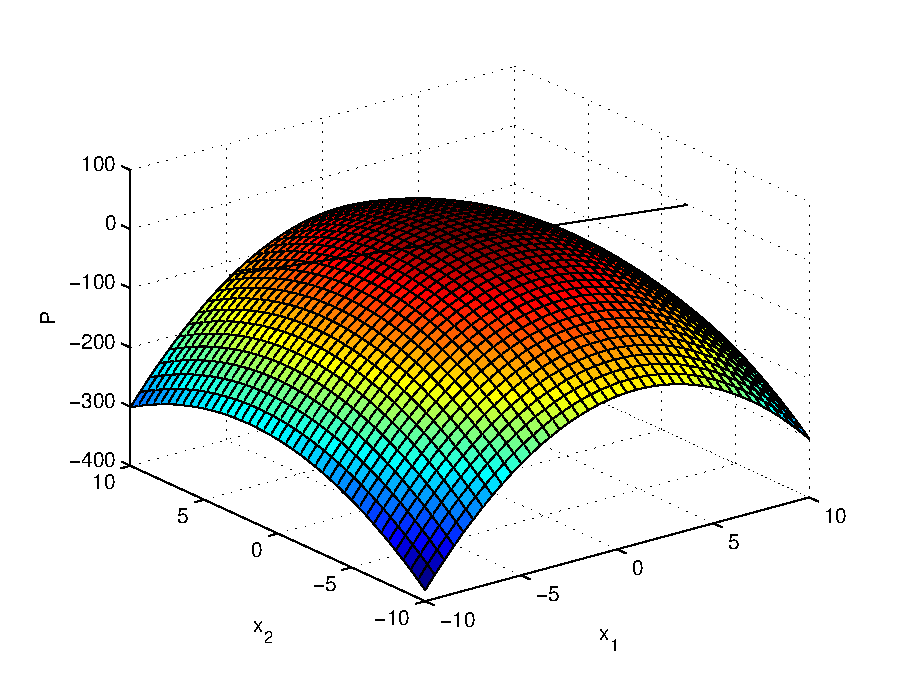
\includegraphics[keepaspectratio=true,width=0.4\linewidth]{MATLAB/optimizechap/lagran1/lagexam1.eps}}
\subfigure[Convex problem]{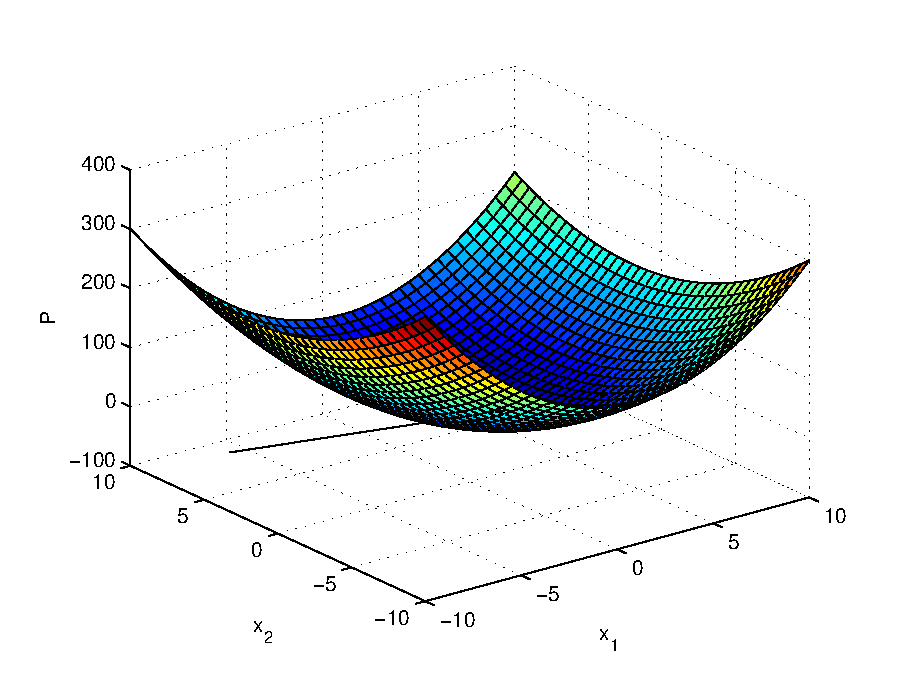
\includegraphics[keepaspectratio=true,width=0.4\linewidth]{MATLAB/optimizechap/lagran1/lagexam2.eps}}
%\caption{Concave Problem : $5-(x_{1}-2)^{2}-2(x_{2}-1)^{2}$}
\label{fig:10-1}
\caption{Convex and concave problem}
\end{figure}

여러개의 구속조건을 갖는 최적화 방식을 일반화 시키면
\begin{equation*}
\begin{aligned}
P : & \underset{x}{\text{maximize}}
& & f(x)\\
& \text{subject to}
& & g_{1}(x)=b_{1}\\
& & & g_{2}(x)=b_{1}\\
& & & \vdots\\
& & & g_{m}(x)=b_{m}\\
\end{aligned}
\end{equation*}
라그랑지안(Lagrangian)을 사용한 해는 다음 식으로 찾을 수 있다.
\begin{equation}
L(x,\lambda)=f(x)+\sum_{i=1}^{m}\lambda_{i}\left(b_{i}-g_{i}(x)\right)
\end{equation}
여기서, $\lambda_{i}$는 $i$번째 구속조건에 관련한 가중치(가격)으로 생각할 수 있다.
\begin{theorem}[Lagrangian multiplier]\label{theo:10-1}
최적화 문제 $P$를 만족시키는 $x^{*}$에 대하여 $x^{*}$와 $\lambda^{*}$가 존재 하고,
$x^{*}=\left(x_{1}^{*},x_{2}^{*},\cdots,x_{n}^{*}\right)$를 함수 $f(x)$를 구속조건 $g_{i}(x)=b_{i},\text{ for }i=1,2,\cdots,m$을 만족시키면서 최대화(maximizes)시키거나 최소화(minimizes)시키는 값을 가지는 벡터로 가정하면,
\begin{itemize}
\item[($i$)] 벡터 $\nabla g_{1}(x^{*}),\nabla g_{2}(x^{*}),\cdots,\nabla g_{m}(x^{*})$가 모두 선형적으로 독립이거나,
\item[($ii$)] $\nabla L(x^{*},\lambda^{*})=0$을 만족시키는 벡터 $\lambda^{*}=\left(\lambda_{1}^{*},\lambda_{2}^{*},\cdots,\lambda_{m}^{*}\right)$가 존재한다.
\end{itemize}
여기서 $\nabla$연산자(Nabla-operator)는 벡터의 편미분 연산자로 다음 식처럼 쓰인다.
\begin{equation}
\nabla = \left(\frac{\partial}{\partial x_{1}},\cdots,\frac{\partial}{\partial x_{n}}\right)
\end{equation}
즉, 위의 라그랑지안 정리는 다음식처럼 쓸 수 있다.
\begin{align}
\frac{\partial L}{\partial x_{1}}\left(x^{*},\lambda^{*}\right)=\frac{\partial L}{\partial x_{2}}\left(x^{*},\lambda^{*}\right)=\cdots=\frac{\partial L}{\partial x_{n}}\left(x^{*},\lambda^{*}\right)=0\\
\frac{\partial L}{\partial \lambda_{1}}\left(x^{*},\lambda^{*}\right)=\frac{\partial L}{\partial \lambda_{2}}\left(x^{*},\lambda^{*}\right)=\cdots=\frac{\partial L}{\partial \lambda_{m}}\left(x^{*},\lambda^{*}\right)=0
\end{align}
\end{theorem}

\subsection{등식과 부등식 구속조건 (Equality and Inequality Constraints)}
등식 구속조건과 부등식 구속조건이 포함된 함수의 최적화는 어떻게 두가지의 조건들을 사용할 수 있느냐에 달려있다. 일반화된 다음 식을 보자.
\begin{equation*}
\begin{aligned}
P : & \underset{x}{\text{maximize}}
& & f(x)\\
& \text{subject to}
& & g_{1}(x)=b_{1}\\
& & & \vdots\\
& & & g_{m}(x)=b_{m}\\
& & & h_{1}(x)\leq d_{1}\\
& & & \vdots\\
& & & h_{p}(x)\leq d_{p}\\
\end{aligned}
\end{equation*}
만약 이 조건이 아닌 $\geq$조건의 경우 $\leq$를 만들어주기 위해 양변에 $-1$을 곱하여 위와 동일한 조건을 만들어준다. 또한 같은 방식으로 최소값 문제는 최대값 문제로 변형할 수 있다.
이 때 라그랑지안은
\begin{equation}
L(x,\lambda,\mu)=f(x)+\sum_{i=1}^{m}\lambda_{i}\left(b_{i}-g_{i}(x)\right)+\sum_{j=1}^{p}\mu_{j}\left(d_{i}-h_{j}(x)\right)
\end{equation}
정리~\ref{theo:10-1}와 유사하게 다음과 같이 정리한다.
$x^{*}=\left(x_{1}^{*},x_{2}^{*},\cdots,x_{n}^{*}\right)$를 함수 $f(x)$를 구속조건 $g_{i}(x)=b_{i},\text{ for }i=1,2,\cdots,m$과 $h_{j}(x)\leq d_{j},\text{ for }j=1,2,\cdots,p$을 만족시키면서 최대화(maximizes)시키는 값을 가지는 벡터로 가정하면,
\begin{itemize}
\item[($i$)] 벡터 $\nabla g_{1}(x^{*}),\cdots,\nabla g_{m}(x^{*})$와 $\nabla h_{1}(x^{*}),\cdots,\nabla h_{p}(x^{*})$가 모두 선형적으로 독립이거나,
\item[($ii$)] 아래의 식을 만족시키는 벡터 $\lambda^{*}=\left(\lambda_{1}^{*},\cdots,\lambda_{m}^{*}\right)$와 $\mu^{*}=\left(\mu_{1}^{*},\cdots,\mu_{p}^{*}\right)$가 존재한다.
\end{itemize}
\begin{align*}
\nabla f(x^{*})-\sum_{i=1}^{m}\lambda_{i}^{*}\nabla g_{i}(x^{*})-\sum_{j=1}^{p}\mu_{j}^{*}\nabla h_{j}(x^{*})&=0\\
\mu_{j}^{*}\left(d_{j}-h_{j}(x^{*})\right)&=0\text{ (Complementarity)}\\
\mu_{j}^{*}&\geq0
\end{align*}
일반적으로 부등식조건이 포함된 해를 구하기 위해서는 우리는 $\mu_{j}^{*}$가 0이 되야하는 조건과 $d_{j}-h_{j}(x_{*})=0$이 되는 상보성(complementarity)조건을 검토해야한다. 이 조건에 만족하는 여러가지 경우의 수에 근거하여 우리는 적절한 하나의 해 혹은 후보해들을 선택해야한다. 만약 최적의 해가 존재한다면, 하나의 해 아니면 후보해들이 그 답이 될 것이다. 위의 조건들은 Kuhn-Tucker(혹은 Karush-Kuhn-Tucker)조건이라고 말한다. KKT조건에서 말하는 것은 최적의 해 $x^{*}$는 부등식 조건에서 꽉 찬 조건이거나 그렇지 않은 경우의 수가 있다. 즉, 부등식 조건에 꽉 찬 조건이 아닌 경우는 무시할 수 있다(해당 경우엔 $\mu_{j}^{*}=0$이 되므로). 그러나 부등식 조건에 꽉 찬 경우는 Lagrangian의 등식조건으로 생각할 수 있기 때문이다.
\begin{equation*}
\mu_{j}^{*}\left(d_{j}-h_{j}(x^{*})\right)=0\text{ (Complementarity)}
\end{equation*}
결국 이 식이 의미하는 것은 최적화 문제에서 부등식조건의 가중치 $\mu_{j}^{*}$를 0으로 잡거나, 구속조건을 꽉 채운 등식조건으로 인식하게 한다.
%\subsubsection{조건의 효용성(Sufficiency of conditions}
%KKT조건(Karush-Kuhn-Tucker conditions)은 적절한 최적해 $x^{*}$의 후보해를 제시해준다. 어떠한 경우에 최적의 충분조건을 
\\
\framebox{예제} \textbf{Complementarity}\\
\rule{\textwidth}{0.1pt}
\begin{equation*}
\begin{aligned}
& \underset{x}{\text{maximize}}& & x^{3}-3x\\
& \text{subject to}& & x\leq2\\
\end{aligned}
\end{equation*}
라그랑지안은
\begin{equation*}
L=x^{3}-3x+\mu(2-x)
\end{equation*}
풀면
\begin{align*}
\frac{\partial L}{\partial x}&=3x^{2}-3-\mu=0\\
x&\leq2\\
\mu(2-x)&=0\\
\mu&\geq0
\end{align*}
2가지의 상보성 조건이 존재한다.
\begin{itemize}
\item 만약 $\mu=0$의 경우에 $3x^{2}-3=0$이 되어 $x=\pm1$이 되고 $f(1)=-2$, $f(-1)=2$가 되기 때문에 해로 적합하다. 
\item 만약 $x=2$라면 $\mu=9$가 된다. 이때도 마찬가지로 $f(2)=2$가 되기 때문에 해로 적합하다.
\end{itemize}
따라서 최대값을 갖는 경우는 2가지의 해를 가지게 된다. $x=-1$과 $x=2$.
\\
\framebox{예제} \textbf{Standard form}\\
\rule{\textwidth}{0.1pt}
\begin{equation*}
\begin{aligned}
& \underset{x,y}{\text{minimize}}& & (x-2)^{2}+2(y-1)^{2}\\
& \text{subject to}& & x+4y\leq 3\\
& & & x\geq y\\
\end{aligned}
\end{equation*}
위의 식을 최대값을 갖는 형태와 표준형태로 변형하면,
\begin{equation*}
\begin{aligned}
& \underset{x,y}{\text{maximize}}& & -(x-2)^{2}-2(y-1)^{2}\\
& \text{subject to}& & x+4y\leq 3\\
& & & -x+y\leq0\\
\end{aligned}
\end{equation*}
라그랑지안은
\begin{equation*}
L(x,y,\mu_{1},\mu_{2})=-(x-2)^{2}-2(y-1)^{2}+\mu_{1}(3-x-4y)+\mu_{2}(0+x-y)
\end{equation*}
풀면 다음 조건이 된다.
\begin{align*}
\frac{\partial L}{\partial x}&=-2(x-2)-\mu_{1}+\mu_{2}=0\\
\frac{\partial L}{\partial y}&=-4(y-1)-4\mu_{1}-\mu_{2}=0\\
\frac{\partial L}{\partial \mu_{1}}&=\mu_{1}(3-x-4y)=0\\
\frac{\partial L}{\partial \mu_{2}}&=\mu_{1}(x-y)=0\\
x+4y&\leq3\\
-x+y&\leq0\\
\mu_{1},\mu_{2}&\geq0
\end{align*}
여기서 총 2개의 상보성 조건이 존재하기 때문에, 우리는 4가지의 경우를 체크해야한다.
\begin{itemize}
\item $\mu_{1}=0$, $\mu_{2}=0$의 경우 $x=2$, $y=1$이 되기 때문에 해로 부적합하다.
\item $\mu_{1}=0$, $x-y=0$의 경우 $x=4/3$, $y=4/3$, $\mu_{2}=-4/3$이 되기 때문에 해로 부적합하다.
\item $\mu_{2}=0$, $3-x-4y=0$의 경우 $x=5/3$, $y=1/3$, $\mu_{1}=2/3$이 되므로 해로 적합하다.
\item $3-x-4y=0$, $x-y=0$의 경우 $x=3/5$, $y=3/5$, $\mu_{1}=22/25$, $\mu_{2}=-48/25$가 되므로 해로 부적합하다.
\end{itemize}
따라서 최적해는 $x=5/3$, $y=1/3$임을 알 수 있다.
%\subsubsection{쿤-터커 정리(Kuhn-Tucker theroem)}
%부등식 조건이 포함된 최적화문제의 1계조건(First Order Condition)에 대한 정리이다. 위의 일반적인 최적화 문제에서 부등식 조건만 생각해보자.
%\begin{equation*}
%\begin{aligned}
%P : & \underset{x}{\text{maximize}}
%& & f(x)\\
%& \text{subject to}& & g_{1}(x)\leq b_{1}\\
%& & & g_{2}(x)\leq b_{2}\\
%& & & \vdots\\
%& & & g_{m}(x)=b_{m}\\
%& & & x_{j}\geq0, j=1,\cdots,n\\
%\end{aligned}
%\end{equation*}
%$(x_{1},x_{2},\cdots,x_{n})$이 원래 모델의 최적해라면, 다음과 같은 조건을 만족시키는 Lagrangian multiplier $\lambda$가 존재한다.
%\begin{align}
%\frac{\partial f}{\partial x_{j}}-\sum_{i=1}^{m}\frac{\partial g_{i}}{\partial x_{j}}&\leq 0, j=1,2,\cdots,n\\
%g_{i}(x_{1},x_{2},\cdots,x_{n})-b_{i}&\leq 0, i=1,2,\cdots,m\\
%x_{j}&\geq0, j=1,2,\cdots,n\\
%\lambda_{i}&\geq0, i=1,2,\cdots,m\\
%\end{align}
\subsection{선형계획모형 해법}
선형계획모형의 해를 구하는 해법으로 도해법(graphical solution)과 대수적 방법(algebraic method)이 있다. 도해법은 의사결정변수가 2개인 경우에 2차원 평면에서 적용될 수 있어 유용하지만, 3개이상인 경우 적용되는데 어려움이 발생하여 일반적인 해법이라고 보기 어렵다. 일반적으로 2개 이상의 변수에서 도해법이 유용한 경우는 고정된 조건에 의해 특성을 알아보려할 때 유용하다. 또한 최적해를 구하는 해법의 특성을 이해하는데에도 필요하다. 보통 변수가 2개를 초과하면 대수적인 방법으로 해를 구해야한다. 대표적인 대수적 방법으로는 Simplex법, 타원체해법(ellipsoid algorithm), 그리고 Karmarkar의 알고리즘이 있다. Simplex법은 1947년 George B, Danzig에 의하여, 타원체해법은 1979년 Khachian에 의하여, Karmarker의 알고리즘은 1984년 Karmarkar에 의하여 개발되었으며 내부점해법(interior-point algorithm)으로도 불린다. 타원체해법은 현재 거의 사용되지 않고 있고, 규모가 큰(large scale) 선형계획모형에 있어서는 근사치를 제고하는 내부점해법(interior-point method)이 Simplex법보다 복잡성 측면에서 우수한 것으로 알려져 있으나 일반적인 규모에서는 Simplex법이 효용성이 인정되어 아직도 널리 사용되고 있다. MATLAB Optimization Toolbox 패키지의 \texttt{linprog}의 함수에서도 규모를 분리하여 내부점해법과 Simplex법을 모두 차용하고 있다.\\
\framebox{문제} \textbf{LP문제 세우기}\\
\rule{\textwidth}{0.1pt}
다음의 문제는 화학공학, 혹은 석유공학분야에서 발생하는 문제이다. 그러나 유한한 자원을 가지고 제품을 생산하는 모든 공학분야에도 적용할 수 있다.\\
가스를 정제하는 공장이 매주 일정한 양의 원료가스를 받는다고 가정한다. 원료가스는 난방용 가스로 사용되는 보통 및 우수 품질의 두 가지 등급으로 정제된다. 이러한 등급들의 가스는 매우 수요가 높으며(항상 잘 팔림), 회사에 각각 다른 이윤을 가져다 준다. 그렇지만 이것들의 생산은 시간과 공장 내의 저장이라는 구속조건을 갖는다. 예를 들면 한 번에 한 개 등급의 제품만이 생산되며, 시설물은 단지 주당 80시간만 사용된다. 또한 각각의 제품들에 대하여 공장 내 보관장소의 제약이 따른다. 이러한 모든 인자들을 아래의 표로 정리되어 있다.
\begin{table}[!hbt]
\centering
\begin{tabular}{c|c|c|c}
\hline\hline
&\multicolumn{2}{c|}{Product}&\\
\cline{2-3}
Resource&Regular&Premium&Resource Availability\\
\hline
Raw gas& $7m^{3}/\text{tonne}$ & $11m^{3}/\text{tonne}$ & $77m^{3}/\text{week}$\\
Production time& $10hr/\text{tonne}$ & $8hr/\text{tonne}$ & $80hr/\text{week}$\\
Storage& $9\text{tonnes}$ & $6\text{tonnes}$ & -\\
\hline
Profit& $150/\text{tonne}$ & $175/\text{tonne}$ & -\\
\hline\hline
\end{tabular}
\end{table}
\\위의 선형프로그래밍문제는 교재에서는 Simplex법을 기초로 설명하고 있다. 일단 이 서술형 문제에서 선형프로그래밍식으로 작성해보자.
공장을 가동하는 기술자는 이윤을 극대화하기 위하여 각각 얼마만큼의 가스들을 생산할지를 결정하여야 한다. 주당 생산되는 보통 등급과 우수 등급의 제품의 양을 각각 $x_{1}$과 $x_{2}$라고 한다면, 주당 전체 이윤은 다음과 같이 계산된다.
\begin{equation*}
\text{total profit per week}=150x_{1}+175x_{2}
\end{equation*}
구속조건들은 비슷한 방법으로 구할 수 있다. 예를 들면 전체 원료가스의 사용량은 다음과 같이 계산된다.
\begin{equation*}
\text{total gas used amount per week}=7x_{1}+11x_{2}
\end{equation*}
이 함계는 주당 가용한 양인 $77m^{3}/week$를 넘지 않아야한다. 따라서 구속조건은 다음 과 같이 표시된다.
\begin{equation*}
7x_{1}+11x_{2}\leq77
\end{equation*}
남은 구속조건들도 같은 방법으로 구해지며, 이를 종합하면 선형프로그래밍식은 다음과 같다.
\begin{equation*}
\begin{aligned}
& \underset{x_{1},x_{2}}{\text{maximize}}& & Z=150x_{1}+175x_{2}&\text{이윤의 극대화}\\
& \text{subject to}& & 7x_{1}+11x_{2}\leq 77&\text{재료의 구속조건}\\
& & & 10x_{1}+8x_{2}\leq 80&\text{시간의 구속조건}\\
& & & x_{1}\leq 9&\text{''보통등급''의 보관 구속조건}\\
& & & x_{2}\leq 6&\text{''우수등급''의 보관 구속조건}\\
& & & x_{1},x_{2}\geq 0&\text{양수의 구속조건}\\
\end{aligned}
\end{equation*}
도해법으로 해를 구하면
\begin{figure}[!hbpt]
\centering
\subfigure[$7x_{1}+11x_{2}\leq 77$]{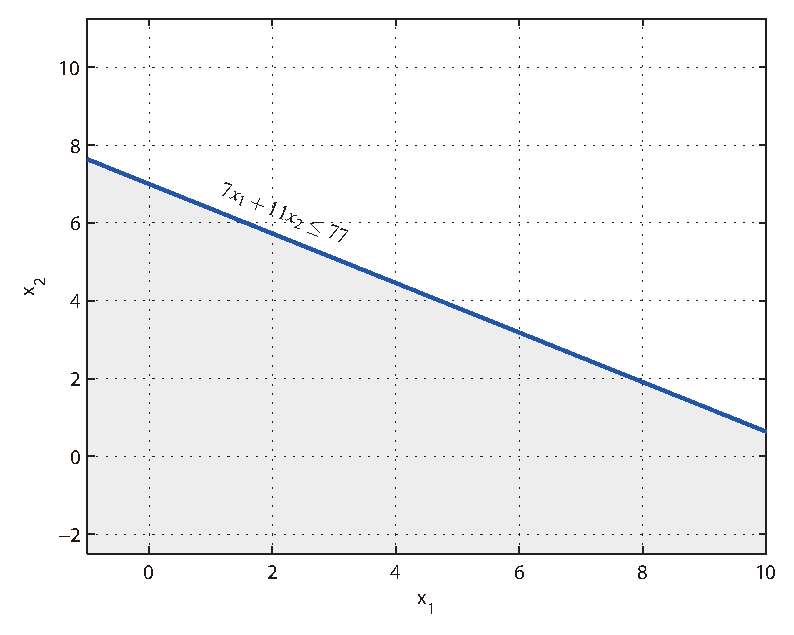
\includegraphics[keepaspectratio=true,width=0.4\textwidth]{MATLAB/optimizechap/lagran1/lin1.eps}}
\subfigure[$10x_{1}+8x_{2}\leq 80$]{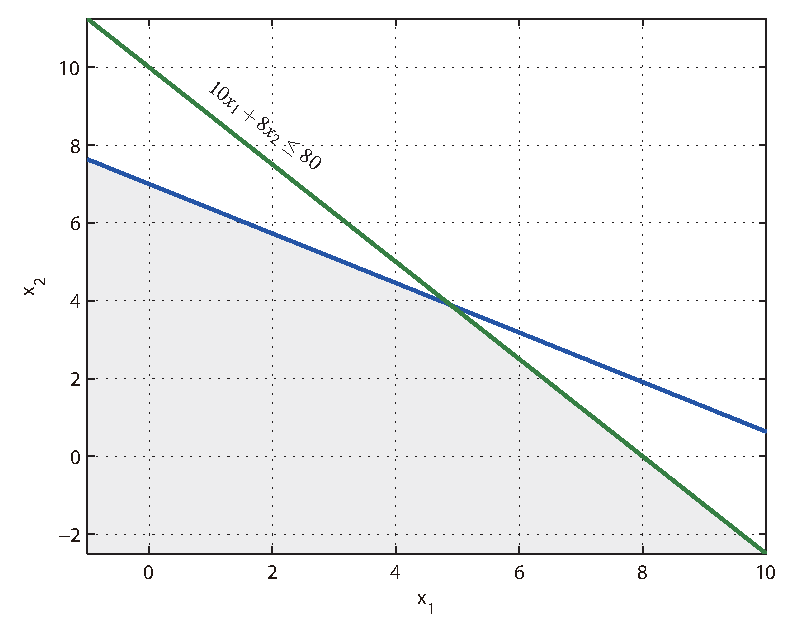
\includegraphics[keepaspectratio=true,width=0.4\textwidth]{MATLAB/optimizechap/lagran1/lin2.eps}}
\subfigure[$x_{2}\leq 6$]{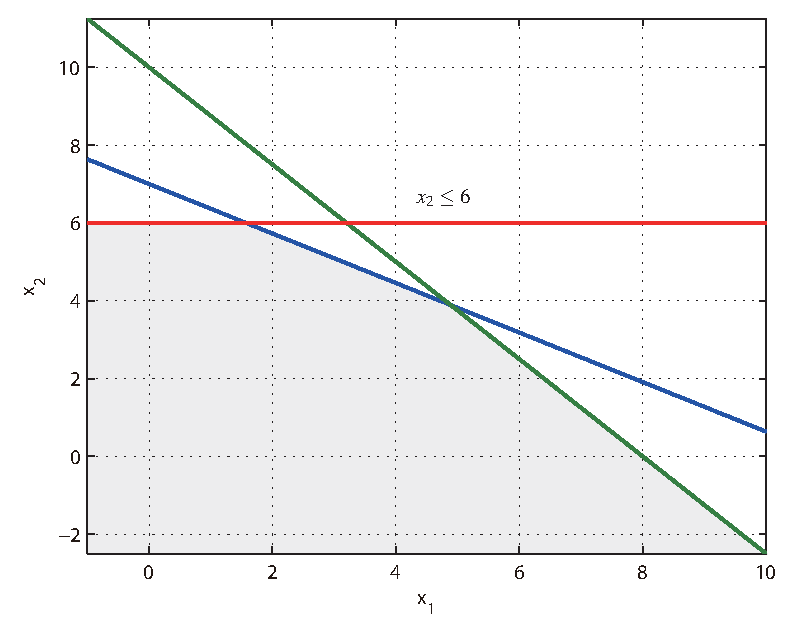
\includegraphics[keepaspectratio=true,width=0.4\textwidth]{MATLAB/optimizechap/lagran1/lin3.eps}}
\subfigure[$x_{1}\leq 9$]{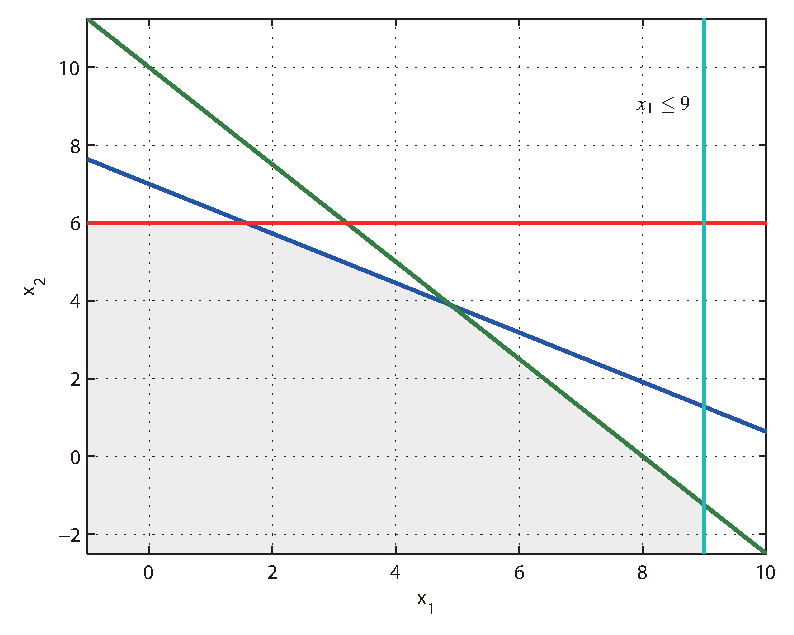
\includegraphics[keepaspectratio=true,width=0.4\textwidth]{MATLAB/optimizechap/lagran1/lin4.eps}}
\subfigure[$x_{1},x_{2}\geq 0$]{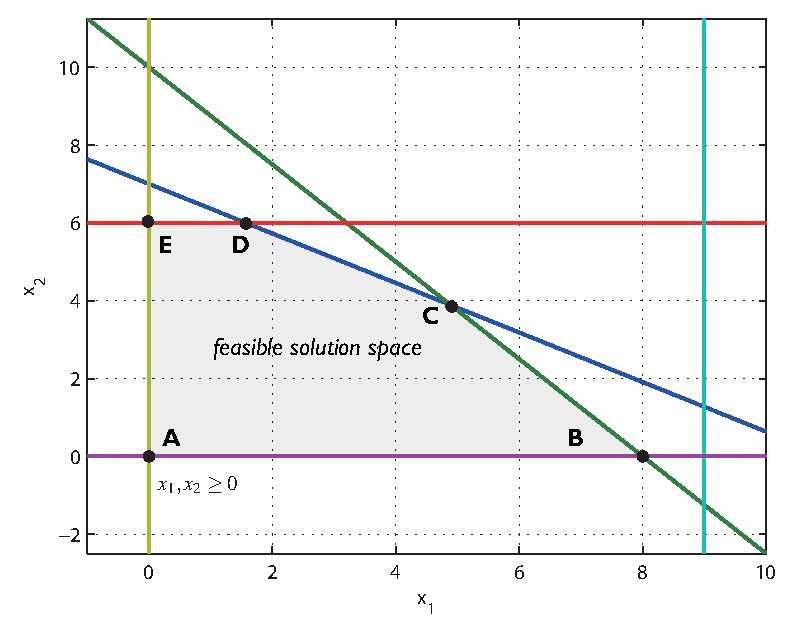
\includegraphics[keepaspectratio=true,width=0.4\textwidth]{MATLAB/optimizechap/lagran1/lin6.eps}}
\subfigure[$Z=150x_{1}+175x_{2}$]{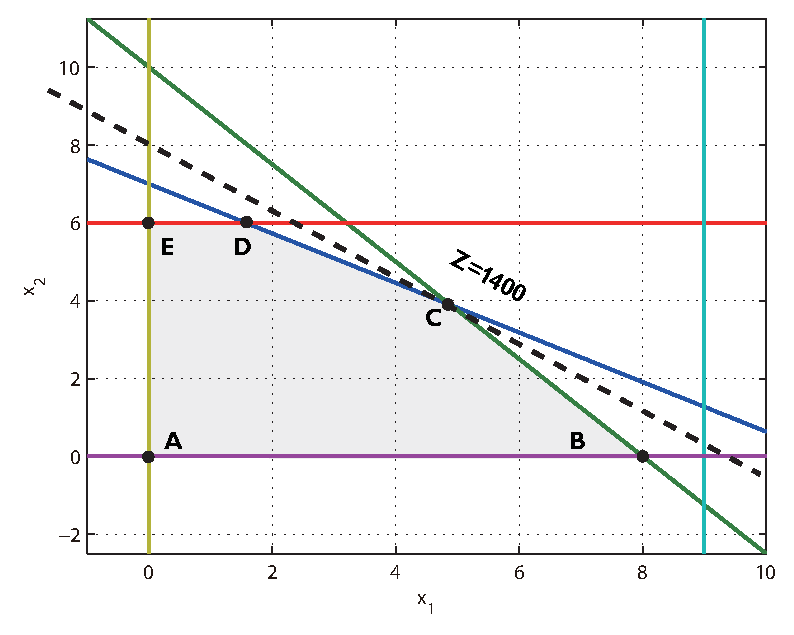
\includegraphics[keepaspectratio=true,width=0.4\textwidth]{MATLAB/optimizechap/lagran1/lin7.eps}}
\caption{Graphical solution}
\label{fig:10-2}
\end{figure}
\clearpage
\subsection{패키지를 사용한 최적화\\(MATLAB Optimization Toolbox Functions)}\label{sec:optoolbox}
다음 테이블은 MATLAB에서 사용할 수 있는 최적화 함수들을 나타낸다. 이 함수들은 최적화 툴박스에서 사용되어지지만 근을 구하거나, 최소화, 그리고 여러개의 목적함수를 둔 최적화 그리고 회귀분석에 이용될 수 있다.
%\subsubsection{Minimization Problems}
%\def\arraystretch{1.7}
\begin{table}[!hbt]
\centering
\begin{tabular}{l|M|l}
\hline\hline
Type&\text{Formulation}&Solver\tabularnewline\hline\hline
Scalar minimization&\begin{array}{cccc} & \underset{x}{\text{min}}&&f(x)\\&\text{subject to}&&l<x<u, (x\text{ is scalar})\end{array}&\texttt{fminbnd()}\tabularnewline\hline

Unconstrained minimization&\begin{array}{cccc} & \underset{x}{\text{min}}&&f(x)\\&\text{subject to}&&(none)\end{array}&\texttt{fminunc()},\texttt{fminsearch()}\tabularnewline\hline

Linear programming&\begin{array}{cccc} & \underset{x}{\text{min}}&&\mathbf{f}^{\top}\mathbf{x}\\&\text{subject to}&&\mathbf{Ax}\leq \mathbf{b}, \mathbf{A}_{eq}\mathbf{x}=\mathbf{b}_{eq},l\leq x\leq u\end{array}&\texttt{linprog()}\tabularnewline\hline

Quadratic programming&\begin{array}{cccc} & \underset{x}{\text{min}}&&\frac{1}{2}\mathbf{x}^{\top}\mathbf{Hx}+\mathbf{c}^{\top}\mathbf{x}\\&\text{subject to}&&\mathbf{Ax}\leq \mathbf{b}, \mathbf{A}_{eq}\mathbf{x}=\mathbf{b}_{eq},l\leq x\leq u\end{array}&\texttt{quadprog()}\tabularnewline\hline

Constrained minimization&\begin{array}{cccc} & \underset{\mathbf{x}}{\text{min}}&&f(\mathbf{x})\\&\text{subject to}&&c(x)\leq0,c_{eq}(x)=0,\\&&&\mathbf{Ax}\leq \mathbf{b}, \mathbf{A}_{eq}\mathbf{x}=\mathbf{b}_{eq},l\leq x\leq u\end{array}&\texttt{fmincon()}\tabularnewline\hline\hline

\end{tabular}
\end{table}
\subsubsection{Linear programming \texttt{lingprog()}}
MATLAB함수의 \texttt{lingprog()}는 선형계획법의 최적해를 구해준다. \texttt{linprog()}함수가 사용하는 알고리즘은 옵션에 선언해 주지 않는 이상 Large scale linear programming과 Medium scale linear programming 으로 자동선택되어 사용되어진다. 디폴트 옵션으로 사용되어지는 Large scale LP는 Mehrotra's predictor-corrector 알고리즘\footnote{Mehrotra, S., "On the Implementation of a Primal-Dual Interior Point Method," SIAM Journal on Optimization, Vol. 2, pp 575–601, 1992.}의 변형인 primal-dual interior-point method를 사용한 LIPSOL\footnote{Zhang, Y., "Solving Large-Scale Linear Programs by Interior-Point Methods Under the MATLAB Environment," Department of Mathematics and Statistics, University of Maryland, Baltimore County, Baltimore, MD, Technical Report TR96-01, July, 1995.}법을 사용한다. Medium scale LP는 1947년 George Dantzig\footnote{George B. Dantzig, "Programming of Interdependent Activities: II Mathematical Model" Econometrica Vol. 17, No. 3/4, pp. 200-211, 1949.}가 개발한 Simplex법(Simplex method)를 사용한다.
\begin{equation*}
\begin{aligned}
& \underset{\mathbf{x}}{\text{minimize}}& & \mathbf{f}^{\top}\\
& \text{subject to}& & \mathbf{A}\cdot\mathbf{x}\leq\mathbf{b}\\
& & & \mathbf{A}_{eq}\cdot\mathbf{x}=\mathbf{b}_{eq}\\
& & & \mathbf{L}_{b}\leq\mathbf{x}\leq\mathbf{U}_{b}\\
\end{aligned}
\end{equation*}
위의 수식은 MATLAB에서 사용할 수 있는 형태로 표현하기 위해, 행렬형태를 사용한다. \\
\texttt{[x,fval,exitflag,output,lambda] = }\textbf{linprog}\texttt{(f,A,b,Aeq,beq,lb,ub,x0,options)}
\begin{table}[!hbt]
\centering
\begin{tabular}{l|l}
\hline\hline
\texttt{f}& Linear objective function vector \texttt{f}\\\hline
\texttt{Aineq}& Matrix for linear inequality constraints\\\hline
\texttt{bineq}& Vector for linear inequality constraints\\\hline
\texttt{Aeq}& Matrix for linear equality constraints\\\hline
\texttt{beq}& Vector for linear equality constraints\\\hline
\texttt{lb}& Vector of lower boundsubVector of upper bounds\\\hline
\texttt{x0}& Initial point for \texttt{x}, active set algorithm only\\\hline
\texttt{solver}& \texttt{'linprog'}\\\hline
\texttt{options}& Options structure created with \texttt{optimset()}\\
\hline\hline
\end{tabular}
\caption{Input Arguments}
\end{table}
앞서 언급한대로 MATLAB프로그램을 수행하면, Large-scale optimization 방식으로 선형프로그래밍의 최적해를 구한다.
\lstinputlisting[language=Matlab, caption= 가스정제공장 수익극대화의 최적해]{MATLAB/optimizechap/lagran1/linprogramex1.m} 